\documentclass[documentclass]{jsarticle}
\usepackage[top=25truemm,bottom=25truemm,left=20truemm,right=20truemm]{geometry}
\usepackage{listings, jlisting, color}
\usepackage[dvipdfmx]{graphicx}
\usepackage{pdfpages}
\usepackage{amsmath}
\usepackage{amssymb, latexsym}
\usepackage{mathtools}
\usepackage{multirow}
\usepackage{color}
\usepackage{ulem}
\usepackage{here}
\usepackage{wrapfig}
\usepackage{tikz}
\usepackage{tcolorbox}
\tcbuselibrary{breakable, skins, theorems}

% 使用する関数の宣言
% (最低限これさえ宣言していれば十分だと思われるものを書いています)
\usetikzlibrary{intersections, calc, arrows, positioning, arrows.meta}


\newcommand{\Add}[1]{\textcolor{red}{#1}}
\newcommand{\Erase}[1]{\textcolor{red}{\sout{\textcolor{black}{#1}}}}
\newcommand{\ctext}[1]{\raise0.2ex\hbox{\textcircled{\scriptsize{#1}}}}

\lstset{
  basicstyle={\small},
  breaklines=true,
  frame=single,
  tabsize=3,
  numbers=left
}

\begin{document}
\title{ソフトウェア設計演習 最終レポート}
\author{222C1021 今村優希}
\maketitle

%\tableofcontents
\clearpage

\newpage

\section{今回のシステム}

今回は下記仕様の「Live Campus」のようなシステムをモデル化する.
システムの大まかな概要を下記に記す.

\begin{tcolorbox}
  \begin{itemize}
    \item 学生は毎学期ごとに、システムから履修登録を行い、許可された講義を受講する。
    履修の可否は、学修細則に基づきシステムが判断する。
    各学期ごとに履修できる科目数には上限があり、同じ時限に重複した科目を履修することはできない。
    \item 学生は、履修登録期間内には何度でも登録、削除、修正(更新)を行うことが出来る。
    \item 学生は、登録した科目と登録可能な科目の時間割をそれぞれ見ることが出来る。
    \item 学生は、自身のこれまでの成績を確認することができる。
    \item 科目には、必修と選択があり、不合格の必修科目があれば履修登録時にシステムが提示し、履修を促す。
    \item 教員は、複数の科目を担当することがあり、システムから各科目の成績を報告する。
    なお、科目担当者は1名とする。
    \item システムは、成績報告期限までに報告していない教員に督促メールを送る。
    なお、成績報告期限の1週間前に成績報告していない教員には、期限を知らせるメールを送るものとする。
  \end{itemize}
\end{tcolorbox}

\section{設計の作成手順}
今回の設計では,分析モデルを作成した後に,設計モデルを作成する手順を取った.

分析モデルでは以下のUML図を作成した.
各UML図が作成し終わると,レビューを行い,後の工程に大きな影響が出ないように工夫を行った.
\begin{itemize}
  \item ユースケース図
  \item ユースケース記述
  \item クラス図
  \item シーケンス図
  \item アクティビティ図
  \item ステートマシン図
\end{itemize}

これらの図を作成し,分析が一定できると,設計モデルの作成に着手した.
設計モデルでは,パターンの適用を駆使し,システムがより現実的になるよう改変を加えた.

\newpage

\section{ユースケース図}
\subsection*{概要}
システムの概要を把握するためにユースケース図を作成した.
今回のシステムの内容から,必要なアクターは
\begin{itemize}
  \item 学生
  \item 教員
\end{itemize}
であると考えた.

学生は「システムにログイン」,「履修登録,削除」等の直接行うユースケースを作成した.
「履修を促す」というシステム側から行われるユースケースを関連付けている.

教員は「システムにログイン」,「成績の報告をする」というユースケースを作成した.
また,学生と同様に成績報告に関する通知を行うユースケースを関連付けている.

\subsection*{作成した図}
レビュー等を通して作成したユースケースが図\ref*{fig:3-1}である.
%ユースケース図の作成結果
\begin{figure}[H]
  \begin{center}
    \includegraphics*[scale=0.5]{figure/3-1.png}
  \end{center}
  \caption{ユースケース図}
  \label{fig:3-1}
\end{figure}

\subsection*{レビュー内容}
ユースケース「履修の可否を確認する」に関して,「学生」と関連をつけた方が良いということで,「履修登録する」にincludeで関連付けた.
また,ユースケース「ログインする」が必要だと思ったので,作成し,他のユースケースと関連をつけた.

概要から「履修修正」という要件があったが,今回のシステムでは履修削除と履修登録を組み合わせて行うと考えた.

\newpage

\section{ユースケース記述}
\subsection*{概要}
上記で作成したユースケースすべてに対してユースケース記述の作成を行った.
ユースケースそれぞれに対して基本系列を作成し,加えて代替系列が必要なユースケースでは適宜作成を行った.

\subsection*{作成した図}
\subsubsection*{1.学生用にログインする}
\begin{figure}[H]
  \includegraphics*[scale=0.4]{figure/4-1.png}
\end{figure}

\subsubsection*{2.履修登録する}
\begin{figure}[H]
  \includegraphics*[scale=0.4]{figure/4-2.png}
\end{figure}

\subsubsection*{3.履修削除する}
\begin{figure}[H]
  \includegraphics*[scale=0.4]{figure/4-3.png}
\end{figure}

\subsubsection*{4.履修修正する}
\begin{figure}[H]
  \includegraphics*[scale=0.4]{figure/4-4.png}
\end{figure}

\subsubsection*{5.時間割を確認する}
\begin{figure}[H]
  \includegraphics*[scale=0.4]{figure/4-5.png}
\end{figure}

\subsubsection*{6.成績を確認する}
\begin{figure}[H]
  \includegraphics*[scale=0.4]{figure/4-6.png}
\end{figure}

\subsubsection*{7.未習得の履修を促す}
\begin{figure}[H]
  \includegraphics*[scale=0.4]{figure/4-7.png}
\end{figure}

\subsubsection*{8.教員用にログインする}
\begin{figure}[H]
  \includegraphics*[scale=0.4]{figure/4-8.png}
\end{figure}

\subsubsection*{9.成績の報告をする}
\begin{figure}[H]
  \includegraphics*[scale=0.4]{figure/4-9.png}
\end{figure}

\subsubsection*{10.成績報告督促を送る}
\begin{figure}[H]
  \includegraphics*[scale=0.4]{figure/4-10.png}
\end{figure}

\subsubsection*{11.成績報告期限メールを送る}
\begin{figure}[H]
  \includegraphics*[scale=0.4]{figure/4-11.png}
\end{figure}

\subsubsection*{12.履修の可否を確認する}
\begin{figure}[H]
  \includegraphics*[scale=0.4]{figure/4-12.png}
\end{figure}

\newpage

\section{クラス図}
\subsection*{概要}
全体のクラス図は図\ref*{fig:5-1}である.
この図に対して,学生,教員それぞれに関係するクラスで分割して物で詳細な関係を分析した.
そのため,\ref*{fig:5-1}における関係に重複度が内藤の不具合があるが,それは分割した詳細な図で行っているため問題ないと考えている.
\begin{figure}[H]
  \begin{center}
    \includegraphics*[scale=0.3]{figure/5-1.png}
  \end{center}
  \caption{クラス図}
  \label{fig:5-1}
\end{figure}

\subsubsection*{ユーザー}
図\ref*{fig:5-2}ではユーザーと,それを管理するための部分をまとめたものである.
\paragraph*{学生クラス}
学生の名前や学生番号が属性として保存されている.
科目の選択や時間割を確認等の動作を行う.

\paragraph*{教員クラス}
教員の名前や教員IDが属性として保存されている.
成績の登録という動作を行う.

\paragraph*{ユーザークラス}
学生と教員のスーパークラスであり,システムのログインというメソッドを共通化して持っている.

\paragraph*{ログイン管理クラス}
ユーザーがログインした際にログを取る等の動作を行うクラスである.

\begin{figure}[H]
  \begin{center}
    \includegraphics*[scale=0.4]{figure/5-2.png}
  \end{center}
  \caption{ユーザーに関するクラス図}
  \label{fig:5-2}
\end{figure}

\subsubsection*{学生}
図\ref*{fig:5-3}では,学生に関する部分をまとめたクラス図である.
\paragraph*{時間割}
学生毎に時間割が作成される.
履修クラスを参考にしながら時間割を作成し,時間割を表示するという動作を行う.

\paragraph*{科目検索と科目一覧クラス}
学生が科目を検索する際に行うクラスである.
学生が曜日と時間を指定すると科目一覧クラスと連携して条件に合う科目を一覧として表示する.

\paragraph*{履修クラス}
履修クラスはある学生がどの科目を履修しているかを表すクラスである.学生毎に作成されることを想定している
また,履修登録,削除ができるかも確認をする.
このクラスで時間割を管理することを想定している.
成績クラスを参照し,成績も一緒に保存することを想定する.

\paragraph*{修得管理クラス}
履修クラスで履修状況を確認し,修得できていなかったら修得を促すクラスである.

\begin{figure}[H]
  \begin{center}
    \includegraphics*[scale=0.4]{figure/5-3.png}
  \end{center}
  \caption{学生に関するクラス図}
  \label{fig:5-3}
\end{figure}

\subsubsection*{教員}
図\ref*{fig:5-4}では,教員に関する部分をまとめたクラス図である.

\paragraph*{科目クラス}
教員は複数の科目を担当することから,教員と関連をつけている.
このクラスは学生と直接かかわりがないが,科目一覧等で間接的に関連付けることで履修等の情報を取れるようにしている.
また,科目には必修,選択必修,選択の3種類の分類がされ,学生毎に科目の立ち位置も変わることから属性に追加するようにした.

\paragraph*{担当科目一覧クラス}
教員が担当している科目を一覧として表示するクラスである.
一人の教員に対して一つの担当科目一覧があることから1対1対応をしている.

\paragraph*{履修者一覧クラス}
担当科目一覧で受け取った科目の履修者一覧を表示するためのクラスである.
このクラスは履修クラスから作成,管理されることを想定している.

\paragraph*{成績関連クラス}
成績クラスは学生,科目毎にオブジェクトが作成されることを想定したクラス図である.
このクラスを基に成績表クラスが作成,管理されている.
また,成績クラスには,未登録,仮登録,本登録という教員の成績登録状況を持っている.
その状況を基に教員に通知を行う報告管理クラスが関連づいている.

\begin{figure}[H]
  \begin{center}
    \includegraphics*[scale=0.4]{figure/5-4.png}
  \end{center}
  \caption{教員に関するクラス図}
  \label{fig:5-4}
\end{figure}

\subsection*{レビュー内容}
\begin{itemize}
  \item クラス図間の関連が複雑で,必要のない部分まで関連付けていたためかなりの省略を加えた.
  \item 重複度が登録されていない部分があったので加えた.
  \item 履修クラスに対して多くのメソッドがあり,責任が大きすぎたので他のクラスを作成することで責任をできるだけ小さくした.
  \item 教員の成績登録の方法がシーケンス図等を通して変更されたことから,クラス図にも適用した.
  \item 科目に必修等の分類があることから継承したクラスを新たに作成した.
\end{itemize}

\newpage

\section{シーケンス図}
\subsection*{概要}
作成したシーケンス図は,
\begin{itemize}
  \item 図\ref*{fig:6-1}: ログイン時のシーケンス図
  \item 図\ref*{fig:6-2}: 履修登録,削除のシーケンス図
  \item 図\ref*{fig:6-3}: 時間割確認のシーケンス図
  \item 図\ref*{fig:6-5}: 修得を促すのシーケンス図
  \item 図\ref*{fig:6-4}: 成績を確認,登録のシーケンス図
  \item 図\ref*{fig:6-6}: 成績報告メールのシーケンス図
\end{itemize}
である.


\subsection*{作成した図}
\subsubsection*{ログイン}
ユーザーという学生,教員ともにログインを行う.
IDとPasswordをユーザーが確認し,ログイン管理が確認を行っている.

\subsubsection*{履修登録,削除}
履修登録,削除をまとめて行うように工夫を行った.
学生が選択した科目が履修登録されていなかった場合は履修登録をし,されていた場合は削除するというシーケンスにした.
ユースケースやシステム概要には履修修正というものがあったが,今回のシステムは履修削除と登録を組み合わせて行うことからシーケンス図の作成は省略した.

%シーケンス図の表示
\begin{figure}[H]
  \centering
  \begin{minipage}[b]{0.49\columnwidth}
      \centering
      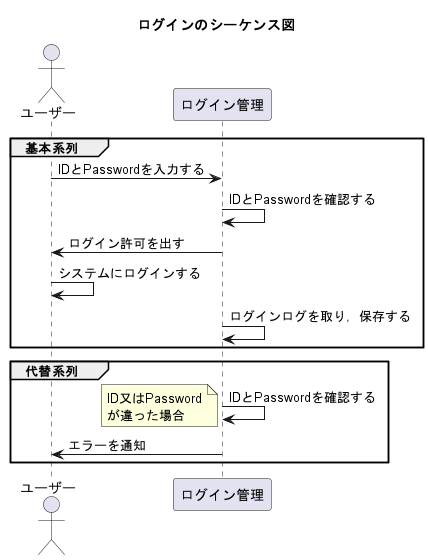
\includegraphics[width=0.8\columnwidth]{figure/6-1.png}
      \caption{ログイン時のシーケンス図}
      \label{fig:6-1}
  \end{minipage}
  \begin{minipage}[b]{0.49\columnwidth}
      \centering
      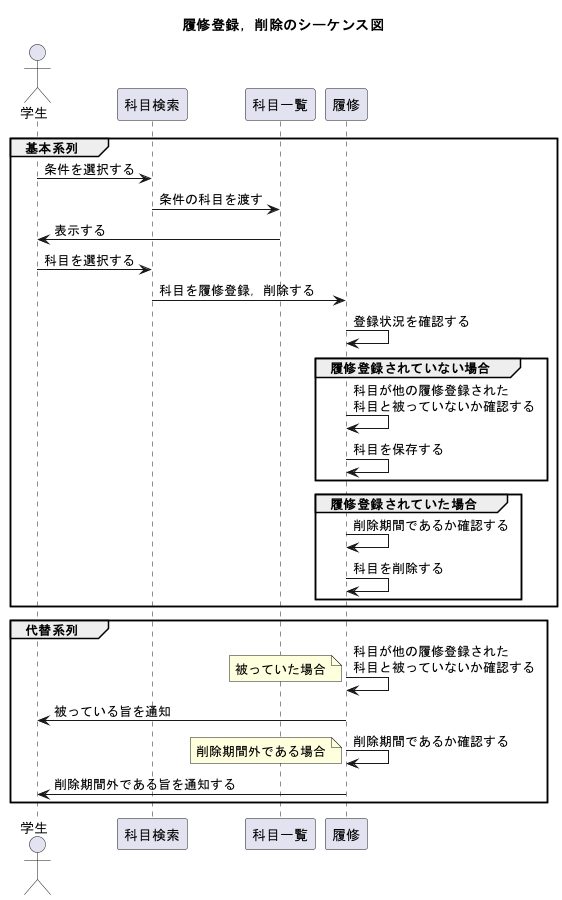
\includegraphics[width=1.0\columnwidth]{figure/6-2.png}
      \caption{履修登録,履修削除のシーケンス図}
      \label{fig:6-2}
  \end{minipage}
\end{figure}

\subsubsection*{時間割}
履修クラスを反映し時間割を作成することから,シーケンス図を作成した.
システム側は事前に時間割を作成しており,学生はそれを確認するのみと想定している.

\subsubsection*{履修を促す}
システム側が履修と必修を確認し,必修が修得されていなかった場合に修得を促す通知を出すと想定している.

\begin{figure}[H]
  \centering
  \begin{minipage}[b]{0.49\columnwidth}
      \centering
      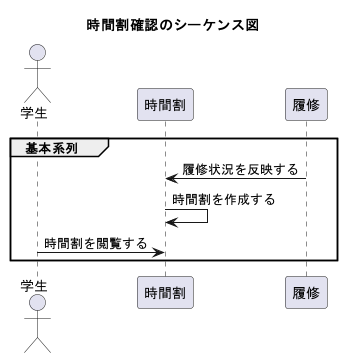
\includegraphics[width=0.7\columnwidth]{figure/6-3.png}
      \caption{時間割確認のシーケンス図}
      \label{fig:6-3}
  \end{minipage}
  \begin{minipage}[b]{0.49\columnwidth}
      \centering
      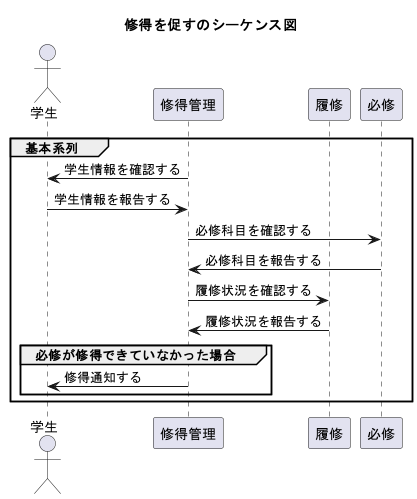
\includegraphics[width=0.7\columnwidth]{figure/6-5.png}
      \caption{修得を促すシーケンス図}
      \label{fig:6-5}
  \end{minipage}
\end{figure}

\subsubsection*{成績}
教員が担当科目一覧から科目を選択し,その科目の履修者一覧をシステムが表示する.
そこで教員が成績を入力し,システムが保存をしている.
その保存された成績を基に成績表をシステムが作成し,学生はそれを閲覧するのみである.

\begin{figure}[H]
  \begin{center}
    \includegraphics*[scale=0.5]{figure/6-4.png}
  \end{center}
  \caption{成績を確認,登録のシーケンス図}
  \label{fig:6-4}
\end{figure}

\paragraph*{成績報告}
成績報告のステータスを確認し,もし成績が登録されていなかった場合,期間ごとに操作が異なる.
一週間前の場合は報告期限を通知し,提出期限を超えていた場合は提出の督促を通知している.

\begin{figure}[H]
  \begin{center}
    \includegraphics*[scale=0.5]{figure/6-6.png}
  \end{center}
  \caption{成績報告メールのシーケンス図}
  \label{fig:6-6}
\end{figure}

\subsection*{レビュー内容}
\begin{itemize}
  \item 履修登録,削除を同じシーケンスで表せるような動作にするよう工夫を行った.
  \item 時間割や成績確認では,システムが作成し,学生が確認できる状態に変更した.
  \item 複数のシーケンス図では流れが変だったので変更を加えた.
\end{itemize}

\newpage

\section{アクティビティ図}
\subsection*{概要}
作成したアクティビティ図は,
\begin{itemize}
  \item 図\ref*{fig:7-1}: ログインするのアクティビティ図
  \item 図\ref*{fig:7-2}: 履修登録,削除のアクティビティ図
  \item 図\ref*{fig:7-3}: 時間割を確認のアクティビティ図
  \item 図\ref*{fig:7-4}: 成績を確認のアクティビティ図
  \item 図\ref*{fig:7-5}: 成績を登録するのアクティビティ図
  \item 図\ref*{fig:7-6}: 未修得の履修を促すのアクティビティ図
  \item 図\ref*{fig:7-7}: 成績報告の通知を出す
\end{itemize}
である.

\subsection*{作成した図}
\subsubsection*{ログイン}
今回は学生のみで作成しているが,教員でも同じ動作をする.
学生が入力したID,Passwordをシステムが正しいか確認し,それぞれで動作が異なる.

\begin{figure}[H]
  \begin{center}
    \includegraphics*[scale=0.4]{figure/7-1.png}
  \end{center}
  \caption{ログインするのアクティビティ図}
  \label{fig:7-1}
\end{figure}

\paragraph*{履修登録,削除}
学生が曜日,時間を選択し,システムが条件にあう科目を表示する.
学生がその科目を選択することで,その科目の状況によって動作が異なる.
それぞれ登録や削除ができるかを確認し,エラーの場合はエラーを表示する動作を行う.

\begin{figure}[H]
  \begin{center}
    \includegraphics*[scale=0.4]{figure/7-2.png}
  \end{center}
  \caption{履修登録,削除のアクティビティ図のアクティビティ図}
  \label{fig:7-2}
\end{figure}

\subsubsection*{時間割,成績}
システムが時間割や成績を作成し,学生がそれを確認している.

\begin{figure}[H]
  \centering
  \begin{minipage}[b]{0.49\columnwidth}
      \centering
      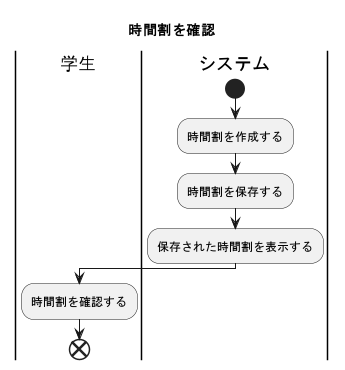
\includegraphics[width=0.8\columnwidth]{figure/7-3.png}
      \caption{時間割を確認するのアクティビティ図}
      \label{fig:7-3}
  \end{minipage}
  \begin{minipage}[b]{0.49\columnwidth}
      \centering
      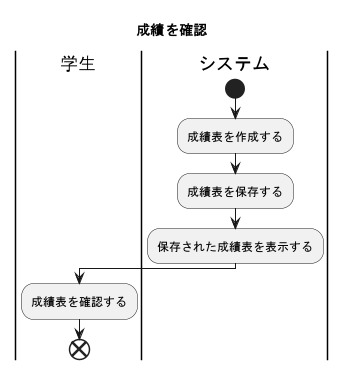
\includegraphics[width=0.8\columnwidth]{figure/7-4.png}
      \caption{成績を確認するのアクティビティ図}
      \label{fig:7-4}
  \end{minipage}
\end{figure}

\subsubsection*{成績を登録}
教員が担当している科目を表示,教員が科目を選択する.
システムはその科目の履修者を表示し,教員がせ成績を入力する.
そのまま教員が保存すると仮成績として保存し,すべての履修者に成績が入力されていた場合,本成績として保存する.

\subsubsection*{未習得の履修}
システムが必修科目や履修状況を確認することで,修得したほうが良いと判断した際に学生に修得を促すようにしている.


\begin{figure}[H]
  \centering
  \begin{minipage}[b]{0.49\columnwidth}
      \centering
      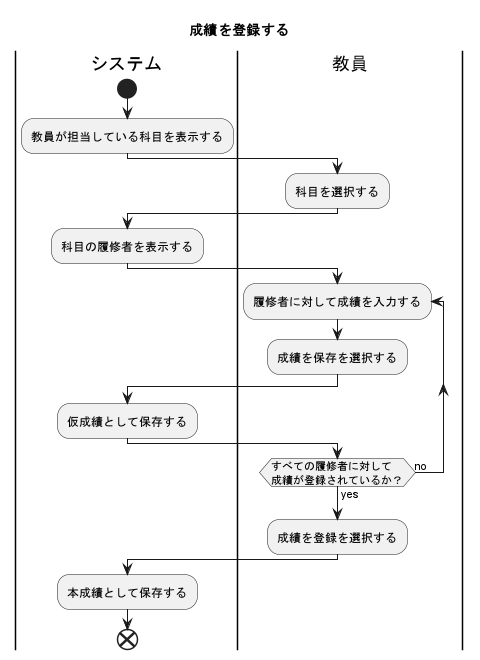
\includegraphics[width=0.9\columnwidth]{figure/7-5.png}
      \caption{成績を登録するのアクティビティ図}
      \label{fig:7-5}
  \end{minipage}
  \begin{minipage}[b]{0.49\columnwidth}
      \centering
      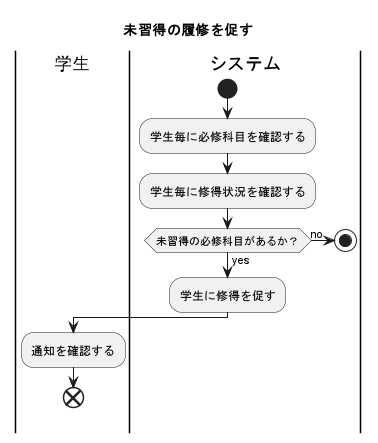
\includegraphics[width=0.8\columnwidth]{figure/7-6.png}
      \caption{未習得の履修を促すのアクティビティ図}
      \label{fig:7-6}
  \end{minipage}
\end{figure}

\subsubsection*{成績報告}
成績報告の期間によって動作が異なる.
すべての履修者に対して成績が登録されていた場合は何も行わないが,登録されていない場合は成績報告の督促等を通知する.

\begin{figure}[H]
  \begin{center}
    \includegraphics*[scale=0.6]{figure/7-7.png}
  \end{center}
  \caption{成績報告の通知を出すアクティビティ図}
  \label{fig:7-7}
\end{figure}
\newpage

\section{ステートマシン図}
\subsection*{概要}
今回のシステムにおいて,「成績」の報告に関してステートマシン図を作成した.


\subsection*{作成した図}
成績は,「未登録状態」→「仮成績」→「本成績」の順で変化する.
その図を図\ref*{fig:8-1}で示す.

\begin{figure}[H]
  \begin{center}
    \includegraphics*[scale=0.6]{figure/8-1.png}
  \end{center}
  \caption{成績のステートマシン図}
  \label{fig:8-1}
\end{figure}

\newpage

\section{設計モデルのクラス図}
作成したクラス図に対して,パターンを導入する等の設計モデルの作成を行った.
また,シーケンス図やステートマシン図等を通して追加したほうが良いと考えたクラス図も追加する作業を行った.

\subsubsection*{ユーザー}
図\ref*{fig:5-2}のユーザーに関するクラス図に対しては,Observerパターンを使用し,ログインの履歴を取る「ログイン管理」クラスがログインを適切に管理できるよう改変を行った.
\begin{figure}[H]
  \begin{center}
    \includegraphics*[scale=0.4]{figure/9-2.png}
  \end{center}
  \caption{設計モデルを適用したログインに関するクラス図}
  \label{fig:9-2}
\end{figure}

\subsubsection*{学生}
図\ref*{fig:5-3}の学生に関するクラス図に関しては,ObserverパターンとStateパターンを用いて設計モデルを作成した.
Observerパターンにおいては,学生の習得状況を取得する際に適用を行った.
Stateパターンは当初のクラス図では使用していなかった,修得状況に対して適用を行った.
修得状況は「必修科目」クラスに関連付けられており,学生それぞれの修得状況によって状態が変更される.
\begin{figure}[H]
  \begin{center}
    \includegraphics*[scale=0.4]{figure/9-3.png}
  \end{center}
  \caption{設計モデルを適用した学生に関するクラス図}
  \label{fig:9-3}
\end{figure}

\subsubsection*{教員}
図\ref*{fig:5-4}の教員に関するクラス図に対しても,ObserverパターンとStateパターンを用いた.
Observerパターンにおいては,教員が成績を報告しているかの管理に対して使用した.
Stateパターンにおいても,教員が成績の報告状況にたいてい使用している.
\begin{figure}[H]
  \begin{center}
    \includegraphics*[scale=0.4]{figure/9-4.png}
  \end{center}
  \caption{設計モデルを適用した教員に関するクラス図}
  \label{fig:9-4}
\end{figure}

\end{document}